
\chapter[Grafos]{Grafos}


\begin{section}{Grafos y sus representaciones}\label{5.1}

Los objetos a los cuales llamaremos {\it {grafos} } son muy útiles
en matemática discreta. Su nombre se deriva del hecho de que
pueden ser entendidos con una notación gráfica (o pictórica), y en
este aspecto solamente se parecen a los familiares gráficos de
funciones que son estudiados en matemática elemental. Pero
nuestros grafos son bastante diferentes de los gráficos de
funciones y están más relacionados con objetos que en el lenguaje
diario llamamos ``redes'' (networks).  \index{redes}

Usaremos la siguiente definición en lo que sigue: dado un conjunto $X$ un {\em $2$-subconjunto} es un subconjunto de $X$ de dos elementos.  

\begin{definicion} Un {\em grafo} $G$ consiste de un  \index{grafo}
conjunto finito $V$, cuyos miembros son llamados
 {\em vértices},  \index{vértices de un grafo}
y un conjunto de $2$-subconjuntos de $V$, cuyos miembros son
llamados {\em aristas}.  \index{aristas de un grafo} Nosotros
usualmente escribiremos $G=(V,E)$ y diremos que $V$ es el {\em
conjunto de vértices} y $E$ es el {\em conjunto de aristas}.
\end{definicion}

La restricción a un conjunto finito no es esencial, pero es
conveniente para nosotros debido a que no consideraremos
``grafos'' infinitos en este apunte.

Un ejemplo típico de un grafo $G=(V,E)$ es dado por los conjuntos
\begin{equation}\label{grafosimple}
V=\{a,b,c,d,z\}, \qquad\quad
E=\{\{a,b\},\{a,d\},\{b,z\},\{c,d\},\{d,z\}\}.
\end{equation}
Este ejemplo y la definición misma no son demasiado
esclarecedores, y solamente cuando con\-si\-de\-ra\-mos la {\it
representación pictórica} de un grafo es cuando se hace la luz.
 \index{representación pictórica (de un grafo)}


\begin{figure}[ht]
	\begin{center}
		\begin{tikzpicture}[scale=1]
		%\SetVertexSimple[Shape=circle,FillColor=white]
		\Vertex[x=0.00, y=2.00]{$a$}
		\Vertex[x=1.90, y=0.62]{$b$}
		\Vertex[x=1.18, y=-1.62]{$c$}
		\Vertex[x=-1.18, y=-1.62]{$d$}
		\Vertex[x=-1.90, y=0.62]{$z$}
		\Edges($c$, $d$,$a$,$b$,$z$,$d$)
		\end{tikzpicture}
	\end{center}	
	\caption{Una representación pictórica del grafo definido en (\ref{grafosimple}).}\label{f5.1}
\end{figure}

Nosotros representamos los vértices como puntos, y unimos dos
puntos con una linea siempre y cuando el correspondiente par de
vértices está en una arista. Luego la Fig. \ref{f5.1} es una
representación pictórica del grafo dado en el ejemplo arriba. Esta
clase de representación es extremadamente conveniente para
trabajar ``a mano'' con grafos relativamente pequeños. Más aún,
esta representación es de gran ayuda para formular y comprender
argumentos abstractos. Nosotros damos a continuación un ejemplo
frívolo.



\begin{figure}[h]
	\begin{center}
		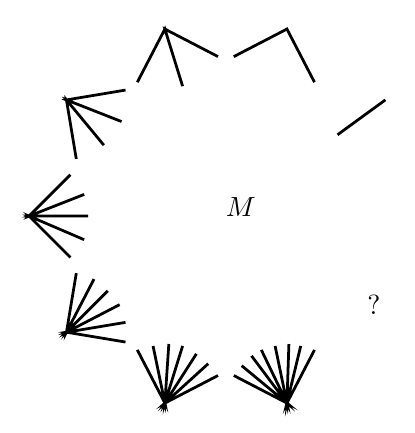
\begin{tikzpicture}[scale=2.5]
		\draw[-,line width=1pt] (0.81,0.59) -- (0.7*0.81,0.7*0.59);
		\draw[-,line width=1pt] (0.31,0.95) -- (0.04, 0.81) -- (0.31,0.95) -- (0.45, 0.68) -- (0.31,0.95);
		\draw[-,line width=1pt] (-0.31,0.95) -- (-0.45, 0.68) -- (-0.31,0.95) -- (-0.22, 0.66) -- (-0.31,0.95) -- (-0.04, 0.81) -- (-0.31,0.95);
		\draw[-,line width=1pt] (-0.81,0.59) -- (-0.76, 0.29) -- (-0.81,0.59) -- (-0.62, 0.36) -- (-0.81,0.59) -- (-0.53, 0.48) -- (-0.81,0.59) -- (-0.51, 0.64) -- (-0.81,0.59);
		\draw[-,line width=1pt] (-1.0,-0.0) -- (-0.79, -0.21) -- (-1.0,-0.0) -- (-0.72, -0.12) -- (-1.0,-0.0) -- (-0.7, -0.0) -- (-1.0,-0.0) -- (-0.72, 0.11) -- (-1.0,-0.0) -- (-0.79, 0.21) -- (-1.0,-0.0);
		\draw[-,line width=1pt] (-0.81,-0.59) -- (-0.51, -0.64) -- (-0.81,-0.59) -- (-0.51, -0.54) -- (-0.81,-0.59) -- (-0.54, -0.45) -- (-0.81,-0.59) -- (-0.6, -0.38) -- (-0.81,-0.59) -- (-0.67, -0.32) -- (-0.81,-0.59) -- (-0.76, -0.29) -- (-0.81,-0.59);
		\draw[-,line width=1pt] (-0.31,-0.95) -- (-0.04, -0.81) -- (-0.31,-0.95) -- (-0.09, -0.75) -- (-0.31,-0.95) -- (-0.15, -0.7) -- (-0.31,-0.95) -- (-0.22, -0.66) -- (-0.31,-0.95) -- (-0.29, -0.65) -- (-0.31,-0.95) -- (-0.37, -0.66) -- (-0.31,-0.95) -- (-0.45, -0.68) -- (-0.31,-0.95);
		\draw[-,line width=1pt] (0.31,-0.95) -- (0.45, -0.68) -- (0.31,-0.95) -- (0.38, -0.66) -- (0.31,-0.95) -- (0.32, -0.65) -- (0.31,-0.95) -- (0.25, -0.66) -- (0.31,-0.95) -- (0.18, -0.68) -- (0.31,-0.95) -- (0.13, -0.71) -- (0.31,-0.95) -- (0.08, -0.76) -- (0.31,-0.95) -- (0.04, -0.81) -- (0.31,-0.95);
		
		\GraphInit[vstyle=Welsh]
		\Vertices[]{circle}{0,1,2,3,4,5,6,7,8,$M$}
		\draw (0.6,-0.45) node {?};
		\end{tikzpicture} 
	\end{center}
	\caption{La fiesta de Abril}\label{f5.2}
\end{figure}


\begin{ejemplo} Mario y su mujer Abril dan una
fiesta en la cual hay otras cuatro parejas de casados. Las
parejas, cuando arriban, estrechan la mano a algunas personas,
pero, naturalmente, no se estrechan la mano entre marido y mujer.
Cuando la fiesta finaliza el profesor pregunta a los otros a
cuantas personas han estrechado la mano, recibiendo $9$ respuestas
diferentes. ?`Cuántas personas estrecharon la mano de Abril?
\end{ejemplo}
\begin{proof}[Solución] Construyamos un grafo cuyos vértices son las personas que asisten a la
fiesta. Las aristas del grafo son las  $\{x,y\}$ siempre y cuando $x$ e $y$ se
hayan estrechado las manos. Puesto que hay nueve personas aparte
de Mario, y que una persona puede estrechar a lo sumo
a otras $8$ personas, se sigue que las $9$ respuestas diferentes que
ha recibido el profesor deben ser $0, 1, 2, 3, 4, 5, 6, 7, 8.$
Denotemos los vértices con estos números y usemos $M$ para Mario. Así obtenemos la representación pictórica de la Fig. \ref{f5.2}


Ahora, el vértice $8$ alcanza a todos los otros vértices excepto
uno, el cual debe por lo tanto representar a la esposa de $8$. Este
vértice debe ser el $0$ el cual por cierto que no está unido al $8$
(ni ob\-via\-men\-te a ningún otro). Luego $8$ y $0$ son una pareja de
casados y $8$ está unido a $1, 2, 3, 4, 5, 6, 7$ y $M$. En particular
el $1$ está unido al $8$ y ésta es la única arista que parte del $1$.
Por consiguiente $7$ no esta unido al $0$ y al $1$ (únicamente), y la
esposa de $7$ debe ser $1$, puesto que $0$ esta casado con $8$.
Continuando con este razonamiento vemos que $6$ y $2$, y $5$ y $3$ son
parejas de casados. Se sigue entonces que $M$ y $4$ están casados,
luego el vértice $4$ representa a Abril, quien estrechó la mano de
cuatro personas.
\end{proof}



Aunque la representación pictórica es intuitivamente atractiva
para los seres humanos, es claramente inútil cuando deseamos
comunicarnos con una computadora. Para lograr esto debemos
re\-pre\-sen\-tar el grafo mediante cierta clase de lista o tabla.
Diremos que dos vértices $x$ e $y$ de un grafo son {\em
adyacentes} cuando $\{x,y\}$ es una arista.
 \index{vértices adyacentes}
(o también diremos que $x$ e $y$ son {\em vecinos}).  Entonces
podemos representar un grafo $G=(V,E)$ por su {\em lista de
adyacencia},  \index{lista de adyacencia} donde cada vértice $v$
encabeza una lista de aquellos vértices que son adyacentes a $v$.
El grafo de Fig. \ref{f5.1} tiene la siguiente lista de
adyacencia:

%\vskip.4cm

\begin{center}
\begin{tabular}{ccccc}
$a$&$b$&$c$&$d$&$z$ \\ \hline
$b$&$a$&$d$&$a$&$b$ \\
$d$&$z$&&$c$&$d$\\
&&&$z$&
\end{tabular}
\end{center}

Las listas de adyacencia son redundantes (cada arista está representada dos veces) pero como todo lenguaje de programación de alto nivel maneja la estructura tipo lista,  preferimos esta representación pues  un grafo  resulta ser como una lista de listas  o un  arreglo de listas.  


\begin{ejemplo}
Por cada entero positivo $n$ definimos el {\em grafo completo  \index{grafo completo}
$K_n$} como el grafo con $n$ vértices y en el cual cada par de vértices es adyacente. 



?`Cuántas aristas tiene $K_n$? De cada vértice ``salen'' $n-1$ aristas, las que van a otros vértices. Si  sumamos $n$-veces las $n-1$ aristas es claro que estamos contando cada arista dos veces, luego el número total de aristas es $n(n-1)/2$ (observar que esta es una demostración, usando  grafos, de que $\sum_{i=1}^n i = n(n-1)/2$).



\end{ejemplo}
%\begin{subsection}{Ejercicios}
\subsection*{\Large $\S$ Ejercicios}
%\addcontentsline{toc}{subsection}{Ejercicios}

\begin{enumerate}
\item A tres casas $A,B,C$ se les debe conectar el gas, el agua y la electricidad: $G,W,E$.
Escribir la lista de adyacencia para el grafo que representa este
problema y construir una representación pictórica del mismo.
?`Puede usted encontrar un dibujo en el cual las líneas que
representan las aristas no se crucen?
\item Los senderos de un jardín han sido diseñados dándoles forma de {\em grafo rueda}
$W_n$, cuyos vértices son $V=\{0,1,2,\ldots,n\}$ y sus aristas son
$$
\begin{aligned}
\{0,1\},\qquad &\{0,2\},\ldots,\{0,n\}, \\
\{1,2\}.\qquad &\{2,3\},\ldots,\{n-1,n\},\qquad \{n,1\}.
\end{aligned}
$$
Describir una ruta por los senderos de tal forma que empiece y
termine en le vértice $0$ y que pase por cada vértice una sola vez.
\item  ?`Para cuales valores de $n$ se puede hacer una representación pictórica
de $K_n$ con la propiedad que las líneas que representan las aristas no se corten?
\item Un {\it {$3$-ciclo}} en un grafo es un conjunto de tres vértices mutuamente adyacentes.
Construir un grafo con cinco vértices y seis aristas que no
contenga $3$-ciclos.
\end{enumerate}
%\end{subsection}

\end{section}



\begin{section}{Isomorfismo de grafos} \label{5.2}
En este punto nosotros debemos enfatizar que un grafo esta
definido como una entidad matemática abstracta. Es en este
contexto que nosotros discutiremos el importante problema de que
queremos decir cuando decimos que dos grafos son ``el
mismo''.

Claramente lo importante de un grafo no son los nombres con que
designamos a los vértices, ni su representación pictórica o
cualquier otra representación. La propiedad característica de un
grafo es la manera en que los vértices están conectados por
aristas. 

Antes de definir isomorfismo de grafos repasaremos el  concepto de función o aplicación biyectiva. Dado  dos conjuntos $X,Y$ diremos que una aplicación $f: X \to Y$ es {\em biyectiva} si para cada $y \in Y$ existe un  único $x \in X$ tal que $f(x) =y$. Un propiedad importante, de las funciones biyectivas es que $f$ es biyectiva si y sólo sí  $f$ tiene {\em inversa}, es decir existe $f^{-1}: Y \to X$, tal que $f(f^{-1}(y)) = y$, $\forall \,y \in Y$ y $f^{-1}(f(x)) = x$, $\forall \,x \in X$.

\begin{ejemplo}
La función  
\begin{align*}
f&: \{1,2,3\}\to\{a,b,c\} \quad \text{definida } f(1) = c, f(2) = b, f(3) = a
\end{align*}
es biyectiva y su  inversa es 
$$
f^{-1}(a) = 3,\;f^{-1}(b) = 2,\;f^{-1}(c) =1.
$$
También es biyectiva la aplicación
\begin{align*}
g&: \{x,y\}\times \{u,w,z\} \to \{1,2,3,4,5,6\} \quad \text{definida } 
\end{align*}
$$
g(x,u)= 1,\, g(x,w) =2,\, g(x,z) =3,\, g(y,u) =4,\, g(y,w) =5,\, g(y,z) =6. 
$$
\end{ejemplo}

\begin{definicion} Dos grafos $G_1$ y $G_2$ se dicen que
son {\em isomorfos} cuando  existe una biyección $\alpha$ entre el
 \index{grafos isomorfos}  \index{isomorfismo de grafos}
conjunto de vértices de $G_1$ y el conjunto de vértices de
$G_2$ tal que  si $\{x,y\}$ es una arista de $G_1$ entonces $\{\alpha(x),\alpha(y)\}$ es una arista de $G_2$ y recíprocamente si  $\{z,w\}$ es una arista de $G_2$ entonces $\{\alpha^{-1}(z),\alpha^{-1}(w)\}$ es una arista de $G_1$. La biyección $\alpha$
es llamada un {\em isomorfismo}.
\end{definicion}

Por ejemplo, considere los dos grafos de la Fig. \ref{f5.3}. En
este caso hay una biyección entre el conjunto de vértices de $G_1$
y el conjunto de vértices de $G_2$ la cual tiene la propiedad
requerida; esta biyección es dada por
$$
\alpha(a)=t,\quad \alpha(b)=v,\quad \alpha(c)=w,\quad \alpha(d)=u.
$$
Podemos comprobar que a cada arista de $G_1$ le corresponde una
arista de $G_2$ y vi\-ce\-ver\-sa. Por ejemplo, a la arista $bc$
de $G_1$ le corresponde la arista $vw$ de $G_2$, y así siguiendo.
(Usaremos la abreviación $xy$ para la arista $\{x,y\}$, recordando
que una arista es un par desordenado, es decir $xy$ es lo mismo
que $yx$.)


\begin{figure}[ht]
	\begin{center}
	\begin{tabular}{llll}
		&
		\begin{tikzpicture}[scale=1]
		%\SetVertexSimple[Shape=circle,FillColor=white]
		\Vertex[x=0,y=0]{$a$}
		\Vertex[x=2,y=0]{$b$}
		\Vertex[x=2,y=-2]{$c$}
		\Vertex[x=0,y=-2]{$d$}
		\Edges($a$, $b$,$c$,$d$,$a$,$b$,$d$)
		\draw (1,-3) node {$G_1$};
		\end{tikzpicture}
		&
		\qquad
		& 
		\begin{tikzpicture}[scale=1]
		%\SetVertexSimple[Shape=circle,FillColor=white]
		\Vertex[x=1,y=0]{$t$}
		\Vertex[x=1,y=-1.3]{$w$}
		\Vertex[x=2,y=-2]{$v$}
		\Vertex[x=0,y=-2]{$u$}
		\Edges($v$, $t$,$u$,$v$,$w$,$u$)
		\draw (1,-3) node {$G_2$};
		\end{tikzpicture}
	\end{tabular}
	\end{center}
	\caption{$G_1$ y $G_2$ son isomorfos} \label{f5.3}
\end{figure}

Cuando, como en la Fig. \ref{f5.3}, dos grafos $G_1$ y $G_2$ son
isomorfos usualmente nos referiremos a ellos como que son ``el
mismo'' grafo.



Para mostrar que dos grafos no son isomorfos, nosotros debemos
demostrar que no hay una biyección entre el conjunto de vértices
de uno con el conjunto de vértices de otro, que lleve las aristas
de uno en las aristas del otro.


\begin{figure}[ht]
	\begin{center}
\begin{tabular}{llll}
	&
	\begin{tikzpicture}[scale=1]
	%\SetVertexSimple[Shape=circle,FillColor=white]
	\Vertex[x=0.00, y=2.00]{$a$}
	\Vertex[x=1.90, y=0.62]{$b$}
	\Vertex[x=1.18, y=-1.62]{$c$}
	\Vertex[x=-1.18, y=-1.62]{$d$}
	\Vertex[x=-1.90, y=0.62]{$e$}
	\Edges($c$, $b$,$a$,$e$,$d$,$b$,$a$,$d$)
	\Edges($e$,$b$)
	\draw (0,-2.2) node {$G_1$};
	\end{tikzpicture}
	&
	\qquad
	& 
	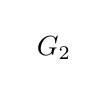
\begin{tikzpicture}[scale=1]
	%\SetVertexSimple[Shape=circle,FillColor=white]
	\Vertex[x=0.00, y=2.00]{1}
	\Vertex[x=1.90, y=0.62]{2}
	\Vertex[x=1.18, y=-1.62]{3}
	\Vertex[x=-1.18, y=-1.62]{4}
	\Vertex[x=-1.90, y=0.62]{5}
	\Edges(1,2,3,4,5,1)
	\Edges(4,2,5)
	\draw (0,-2.2) node {$G_2$};
	\end{tikzpicture}
\end{tabular}
\end{center}
	\caption{$G_1$ y $G_2$ no son isomorfos} \label{f5.4}
\end{figure}

Si dos grafos tienen diferente número de vértices, entonces no es
posible ninguna biyección, y los grafos no pueden ser isomorfos.
Si los grafos tienen el mismo número de vértices, pero di\-fe\-ren\-te
número de aristas, entonces hay biyecciones de vértices  pero ninguna de ellas
puede ser un isomorfismo. 
\begin{definicion} 

Sea $G=(V,E)$ un grafo. Se dice que $G^{\prime}=(V^{\prime},E^{\prime})$ es {\em subgrafo} de
$G=(V,E)$ si $V^{\prime} \subset V$, $E^{\prime} \subset E$ y todos los vértices que son extremos de las aristas de $E^{\prime}$
están en $V^{\prime}$.
\end{definicion}

Es claro, pero  no lo demostraremos aquí, que un isomorfismo lleva un subgrafo a un subgrafo isomorfo. Este resultado es una herramienta que puede ser útil para ver si dos grafos no son isomorfos. 

Por ejemplo, los dos grafos de la Fig. \ref{f5.4} tienen cada uno cinco
vértices y siete aristas pero no son isomorfos. Una manera de ver
esto es observar que los vértices $a$, $b$, $d$, $e$ forman un
subgrafo completo de $G_1$ (cada par de ellos está conectado por
una arista). Cualquier isomorfismo debe llevar estos vértices en
cuatro vértices de $G_2$ con la misma propiedad, y puesto que no
hay tal conjunto de vértices en $G_2$ no puede haber ningún
isomorfismo.


%\begin{subsection}{Ejercicios} 

\subsection*{\Large $\S$ Ejercicios}\label{ejercicios5.2}
%\addcontentsline{toc}{subsection}{Ejercicios}
\begin{enumerate}
\item Probar que los grafos mostrados en la Fig. \ref{f5.5} no son isomorfos.

\begin{figure}[ht]
	\begin{center}
	\begin{tabular}{llll}
		&
		\begin{tikzpicture}[scale=1]
		\SetVertexSimple[Shape=circle,FillColor=white,MinSize=8 pt]
		\Vertex[x=0.00, y=2.00]{a}
		\Vertex[x=2., y=-1.50]{b}
		\Vertex[x=-2., y=-1.50]{c}
		\Edges(a,b,c,a)
		\Vertex[x=0.00, y=0.85]{1}
		\Vertex[x=1., y=-0.9]{2}
		\Vertex[x=-1., y=-0.9]{3}
		\Edges(1,2,3,1)
		\Edges(a,1,3,c,b,2)
		\draw (0,-2.2) node {$G_1$};
		\end{tikzpicture}
		&
		\qquad
		& 
		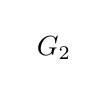
\begin{tikzpicture}[scale=0.65]
		\SetVertexSimple[Shape=circle,FillColor=white,MinSize=8 pt]
		%				
		\Vertex[x=3.00, y=0.00]{1}
		\Vertex[x=1.50, y=2.60]{2}
		\Vertex[x=-1.50, y=2.60]{3}
		\Vertex[x=-3.00, y=0.00]{4}
		\Vertex[x=-1.50, y=-2.60]{5}
		\Vertex[x=1.50, y=-2.60]{6}
		\Edges(1,2,3,4,5,6,1)
		\Edges(1,4) \Edges(3,6) \Edges(2,5)
		\draw (0,-3.8) node {$G_2$};
		\end{tikzpicture}
	\end{tabular}
\end{center}
	\caption{Probar que estos grafos no son isomorfos}\label{f5.5}
\end{figure}

\item \label{ejercicio5.2.2}Encontrar un isomorfismo entre los grafos definidos por las siguientes listas de
adyacencias. (Ambas listas especifican versiones de un grafo
famoso conocido como {\em grafo de Petersen}). \index{grafo de
Petersen}

$$
\begin{matrix}
a&b&c&d&e&f&g&h&i&j\\ \hline
b&a&b&c&d&a&b&c&d&e\\
e&c&d&e&a&h&i&j&f&g\\
f&g&h&i&j&i&j&f&g&h
\end{matrix}
\qquad \begin{matrix}
0&1&2&3&4&5&6&7&8&9\\ \hline
1&2&3&4&5&0&1&0&2&6\\
5&0&1&2&3&4&4&3&5&7\\
7&6&8&7&6&8&9&9&9&8
\end{matrix}
$$

\item Sea $G=(V,E)$ el grafo definido como sigue. El conjunto de vértices $V$ es el conjunto
de todas las palabras de longitud tres en el alfabeto $\{0,1\}$, y
el conjunto de aristas $E$ contiene aquellos pares de palabras que
difieren exactamente en una posición. Probar que $G$ es isomorfo
al grafo formado por las esquinas y aristas de un cubo.
\end{enumerate}
%\end{subsection}


\end{section}



\begin{section}{Valencias}\label{5.3}
La {\em {valencia}} de un vértice $v$ en un grafo $G=(V,E)$ es el
\index{valencia de un vértice} número de aristas de $G$ que contienen a $v$.
Usaremos la notación $\delta(v)$ para la valencia de $v$,
formalmente
$$
\delta(v)=|D_v|, \quad \text{ donde } \quad D_v=\{e \in E| v\in
e\}.
$$
El grafo descrito en Fig. \ref{f5.1} tiene $\delta(a)=2$,
$\delta(b)=2$, $\delta(c)=1$, $\delta(d)=3$, $\delta(z)=2$. El
primer teorema de la teoría de grafos nos dice que la suma de
estos números es dos veces el número de aristas.

\begin{teorema}\label{t5.3} La suma de los valores de las valencias
$\delta(v)$, tomados sobre todos los vértices $v$ del grafo
$G=(V,E)$, es igual a dos veces el número de aristas:
$$
\sum_{v \in V} \delta(v) = 2|E|.
$$
\end{teorema}
\begin{proof} La valencia de un vértice $v$ indica la cantidad de
``extremos'' de aristas que ``tocan'' a $v$. Es claro que hay
$2|E|$ extremos de aristas, luego la suma total de las valencias
de los vértices es $2|E|$.
\end{proof}

Hay un útil corolario de este resultado. Diremos que un vértice de
$G$ es {\em impar} si su  \index{vértice impar}  \index{vértice
par} valencia es impar, y {\em par} si su valencia es par.
Denotemos $V_i$ y $V_p$ los conjuntos de vértices impares y pares
respectivamente, luego $V=V_i \cup V_p$ es una partición de $V$.
Por teorema \ref{t5.3}, tenemos que
$$
\sum_{v \in V_i} \delta(v) + \sum_{v \in V_p} \delta(v)= 2|E|.
$$
Ahora cada término en la segunda suma es par, luego esta suma es
un número par. Puesto que el lado derecho también es un número
par, la primera suma debe ser también par. Pero la suma de números
impares solo puede ser par si el número de términos es par. En
otra palabras:

\begin{teorema} El número de vértices impares es par.
\end{teorema}

Este resultado es a veces llamado el ``handshaking lemma''
(handshake=estrechar la mano, darse la  \index{handshaking lemma}
mano), debido a que se puede interpretar en términos de gente y
darse la mano: dado un conjunto de personas, el número de personas
que le ha dado la mano a un número impar de miembros del conjunto
es par.

Un grafo en el cual todos los vértices tienen la misma valencia
$r$ se llama {\em regular}  \index{grafo regular} (con valencia
$r$), o {\em $r$-valente.} En este caso, el resultado del teorema
\ref{t5.3} se traduce
$$
r|V|=2|E|.
$$

Muchos de los grafos que aparecen en las aplicaciones son
regulares. Ya conocemos los  grafos completos $K_n$; ellos son
regulares, con valencia $n-1$. De geometría elemental conocemos
los polígonos de $n$ lados, los cuales en teoría de grafos son
llamados {\em {grafos cíclicos}}  \index{grafo cíclico} $C_n$.
Formalmente, podemos decir que el conjunto de vértices de $C_n$ es
$\mathbb Z_n$, y los vértices $i$ y $j$ están unidos si $j=i+1$ o
$j=i-1$ en $\mathbb Z_n$. Claramente, $C_n$ es un grafo regular
con valencia $2$, si $n\ge 3$.

Una aplicación importante de la noción de valencia es en el
problema de determinar si dos grafos son o no isomorfos. Si
$\alpha:V_1 \to  V_2$ es un isomorfismo entre $G_1$ y $G_2$, y
$\alpha(v)=w$, entonces cada arista que contiene a $v$ se
transforma en una arista que contiene a $w$. En consecuencia
$\delta(v)=\delta(w)$. Por otro lado, si $G_1$ tiene un vértice
$x$, con valencia $\delta(x)=\delta_0$, y $G_2$ no tiene vértices
con valencia $\delta_0$, entonces $G_1$ y $G_2$ no pueden ser
isomorfos. Esto nos da otra manera para distinguir los grafos de
la Fig \ref{f5.4}, puesto que el primer grafo tiene un vértice de
valencia 1 y el segundo no.

Una extensión de esta idea se da en la siguiente proposición.


\begin{proposicion}\label{criterioiso}Sean  $G_1$ y $G_2$ grafos isomorfos. Para cada $k\ge 0$ sea $n_i(k)$ el
número de vértices de $G_i$ que tienen valencia $k$ ($i=1,2$).
Entonces $n_1(k)=n_2(k)$.
\end{proposicion}
\begin{proof} Hemos visto más arriba que si $\alpha:V_1 \to  V_2$ es un isomorfismo entre $G_1$ y $G_2$ y $v\in V_1$, entonces $\delta(v)=\delta(\alpha(v))$. Luego la cantidad de vértices con valencia $k$ en $G_1$ es igual  a la cantidad de vértices con valencia $k$ en $G_2$.     
\end{proof}

\begin{ejemplo} Revisemos los grafos de la Fig. \ref{f5.4} y la Fig. \ref{f5.5} de la sección anterior. 

Los dos grafos de la Fig. \ref{f5.4}  no son isomorfos debido a que en el primer grafo existen tres vértices con valencia $3$ mientras que en el segundo existen sólo dos.


Observar que los criterios vistos hasta ahora relativos a cantidad de vértices,  cantidad de aristas y valencias, incluyendo el de la proposición \ref{criterioiso}, no son útiles para determinar si los grafos de  la Fig. \ref{f5.5} son isomorfos o no: ambos tienen $6$ vértices, $9$ aristas y todos los vértices son de valencia $3$. Sin embargo, en el caso de la Fig. \ref{f5.5} podemos determinar que los grafos no son isomorfos observando los subgrafos de cada uno. Ahora bien, no  hay ningún criterio general eficiente para determinar si dos grafos son isomorfos o no: en los casos difíciles esencialmente debemos probar con todas las biyecciones posibles de los vértices de un grafo a los vértices del otro y eso es no computable para casos no demasiado  grandes.   
  
 
\end{ejemplo}

%\begin{subsection}{Ejercicios}
\subsection*{\Large $\S$ Ejercicios}\label{ejercicios5.3}
%\addcontentsline{toc}{subsection}{Ejercicios}
\begin{enumerate}
\item ¿Es posible que las siguientes listas sean las valencias de todos los vértices de un
grafo? Si así lo fuera, dar una representación pictórica de tal
grafo. (Recordar que hay a lo más una arista que una un par de
vértices dados.)
\begin{multicols}{2}
	\begin{enumerate}
		\item $2,2,2,3.$
		
		\item $1,2,2,3,4.$
		
		\item $2,2,4,4,4.$
		
		\item $1,2,3,4.$
	\end{enumerate}
\end{multicols}
%
%
%
%$$
%\begin{aligned}
%\text{(i)} \,\,\, 2,2,2,3. \qquad &\text{(ii)} \,\,\, 1,2,2,3,4. \\
%\text{(iii)} \,\,\,2,2,4,4,4. \qquad &\text{(iv)} \,\,\, 1,2,3,4.
%\end{aligned}
%$$
\item Si $G=(V,E)$ es un grafo, el {\em complemento}\index{complemento de un grafo} $G^c$ de $G$ es el grafo cuyo conjunto de
vértices es $V$ y cuyas aristas unen aquellos vértices que no son
unidos por $G$. Si $G$ tiene $n$ vértices y sus valencias son
$d_1,d_2,\ldots,d_n$, ?`cuáles son las valencias de $G^c$?
\item Encuentrar todos los grafos posibles (no isomorfos) que pueda, que sean regulares,
$4$-valentes y con $7$ vértices. [Ayuda: considere el complemento de esos grafos.]

\item Probar que si $G$ es un grafo con al menos dos vértices, entonces $G$ tiene dos
vértices con la misma valencia.
\end{enumerate}

%\end{subsection}

\end{section}




\begin{section}{Caminos y ciclos}\label{5.4}

Frecuentemente usamos grafos como modelos de situaciones prácticas
que involucran rutas: los vértices representan ciudades o cruces,
y cada arista representa una ruta o cualquier otro forma de
comunicación. Las definiciones de esta sección se comprenderán
mejor con esta clase de ejemplo en mente.

\begin{definicion} \rm Una {\em caminata} en un grafo $G$ es  \index{caminata}
una secuencia de vértices
$$
v_1,v_2,\ldots,v_k,
$$
tal que $v_i$ y $v_{i+1}$ son adyacentes ($1 \le i \le k-1$). Si
todos los vértices son distintos, una caminata es llamada un {\em
camino}.  \index{camino}

Llamaremos {\em ciclo} a una caminata \index{ciclo}
$v_1,v_2,\ldots,v_{r+1}$  con $r \ge 3$ y cuyos vértices son distintos exceptuando
los extremos, es decir que $v_1,v_2,\ldots,v_{r}$ es un camino de al menos tres vértices y $v_1=v_{r+1}$.  A menudo diremos que es un {\em
$r$-ciclo}, o un ciclo de {\em longitud} $r$ en $G$.
 \index{longitud de un ciclo}
\end{definicion}

Es decir, una caminata especifica una ruta en $G$: del primer
vértice vamos a uno adyacente, de éste a otro adyacente y así
siguiendo. En una caminata podemos visitar cualquier vértice
varias veces, y en particular, podemos ir de un vértice $x$ a otro
$y$ y luego tomar la dirección contraria y regresar a $x$. En un
camino, cada vértice es visitado solo una vez.

Escribamos $x \sim y$ siempre y cuando los vértices $x$ e $y$ de
$G$ puedan ser unidos por un camino en $G$: hablando en forma
rigurosa, esto significa que hay un camino $v_1,v_2,\ldots,v_k$ en
$G$ con $x=v_1$ e $y=v_k$. 

\begin{lema} Sea $G$ un grafo. $x \sim y$ si  y sólo si $x$ e $y$ pueden ser unidos por una caminata 
\end{lema}
\begin{proof}Es claro que si $x$ e $y$ están unidos por un camino, como  un camino es un caso especial de caminata, $x$ e $y$ están unidos por una caminata.

Veamos que si  $x$ e $y$ están unidos por una caminata, entonces están unidos por un camino. Sea 
$$
x=x_1,x_2,\ldots,x_k=y,
$$
una caminata entre  $x$ e $y$. Si ninguno de los $x_i$ se repite, entonces tenemos un camino y terminado el problema. Si hay repetición, entonces existe $j$ tal que $x_j = x_{j+r}$ con $r >0$, es decir tenemos una caminata
$$
x=x_1,x_2,\ldots,x_j,\ldots,x_{j+r},\ldots, x_k=y,
$$
Como $x_j = x_{j+r}$ podemos eliminar la subcaminata $x_{j+1},\ldots,x_{j+r}$ (un ``bucle'' dentro de la caminata) y nos queda 
$$
x=x_1,x_2,\ldots,x_j,x_{j+r+1},\ldots, x_k=y,
$$
una caminata, más corta,  entre $x$ e $y$. Podemos repetir este procedimiento hasta eliminar todos los ``bucles'' y obtener un camino.
\end{proof}

\begin{definicion} Diremos que un grafo  $G$ es \textit{conexo} si para cualesquiera dos vértices $x,y$ existe una camina de $x$ a $y$, es decir si  $x \sim y$. 
\end{definicion}

Debido al lema que probamos más arriba, es sencillo verificar la siguientes propiedades: sea $G$ grafo y sean $x,y,z$ vértices de $G$, entonces
\begin{enumerate}[label=(\alph*)]
\item  $x \sim x$ (reflexividad de $\sim$).
\item  $x \sim y$, entonces $y \sim x$ (simetría de $\sim$).
\item  $x \sim y$,  $y \sim z$, entonces  $x \sim z$ (transitividad  de $\sim$).
\end{enumerate}


En un lenguaje formal, una relación que  cumple las tres propiedades anteriores es llamada una  {\em relación de equivalencia} del conjunto, en este caso tenemos una relación de equivalencia del conjunto de vértices $V$ de $G$. 

Estas tres propiedades nos permiten partir a $V$ en conjuntos disjuntos: dos vértices están en el mismo conjunto si ellos pueden
ser unidos por un camino, y están en conjuntos diferentes si no podemos encontrar tal camino. llamaremos a estos conjuntos disjuntos las {\em clases de equivalencia de $\sim$}.

\begin{definicion}Supongamos que $G=(V,E)$ es un grafo y
que la partición de $V$ en las clases de equivalencia de $\sim$ es
$$
V= V_1 \cup V_2 \cup \cdots \cup V_r.
$$
Denotemos con $E_i$ ($1\le i \le r$) al subconjunto de $E$ que
contiene todas las aristas cuyos finales están en $V_i$. Entonces
los grafos $G_i=(V_i,E_i)$ son llamados las {\em componentes}  \index{componente de un grafo}  \index{grafo conexo}
de $G$. Si $G$ tiene solo una componente entonces, claramente, el grafo es {conexo}.
\end{definicion}



\begin{figure}[t]
	\begin{center}
\begin{tikzpicture}[scale=1.1]
\SetVertexSimple[Shape=circle,FillColor=white,MinSize=8 pt]			
\Vertex[x=6, y=-0.5]{1}
\Vertex[x=5.5, y=-2]{2}
\Vertex[x=7, y=-3.5]{3}
\Vertex[x=7, y=-2]{4}
\Vertex[x=11, y=-2]{5}
\Vertex[x=6.50, y=-1.2]{6}
\Vertex[x=6.50, y=-2.5]{7}
\Vertex[x=9.5, y=-0.8]{8}
\Vertex[x=8.5, y=-2.5]{9}
\Vertex[x=10, y=-3.3]{a}
\Edges(5,1,2,4,5,3,2,4,3,5,4)
\Edges(a,8,9,7,6,8,9)
\end{tikzpicture}
\end{center}
\caption{Un grafo con dos componentes} \label{f5.6}
\end{figure}

La terminología casi explica por si misma el significado de estas
definiciones. El grafo mostrado en la Fig. \ref{f5.6} tiene dos
componentes, y por consiguiente no es conexo. La descomposición de
un grafo en componentes es muy útil, puesto que muchas propiedades
de los grafos pueden ser establecidas considerando las componentes
separadamente. Por esta razón, teoremas acerca de grafos a menudo
son probados solo para la clase de grafos conexos.

Cuando un grafo de moderado tamaño es dado por una representación
pictórica es bastante fácil determinar si es o no conexo. Sin
embargo, cuando un grafo es dado por una lista de adyacencia
necesitaremos un algoritmo eficiente para decidir si es o no
conexo. 


\begin{figure}[b]
	\begin{center}
		\begin{tikzpicture}[scale=1]
		%\SetVertexSimple[Shape=circle,FillColor=white]
		\def\rvar{1.2}
		\Vertex[x=0.00, y=-2.00]{$u$}
		\Vertex[x=\rvar*1.90, y=-0.62]{$t$}
		\Vertex[x=\rvar*1.18, y=1.62]{$q$}
		\Vertex[x=-1.18*\rvar, y=1.62]{$p$}
		\Vertex[x=-1.90*\rvar, y=-0.62]{$r$}
		\Vertex[x=0, y=0]{$s$}
		\Edges($u$,$t$,$q$,$p$,$r$,$u$,$s$,$t$,$r$,$s$,$q$,$r$,$p$,$t$,$s$,$u$,$s$,$p$)
		\end{tikzpicture}
	\end{center}
	\caption{El gran tour} \label{f5.7}
\end{figure}

\begin{ejemplo}\label{chunner} Leandro y Juan, dos amigos, planean tomar sus vacaciones en determinada isla. La Fig. \ref{f5.7} representa los lugares de interés
turístico de la isla y las carreteras que los unen. Leandro es un turista por naturaleza, y desea visitar cada lugar una vez y volver al punto de partida. Juan es un
explorador, y desea atravesar todos los caminos solo una vez, a él lo tiene sin cuidado si regresa o no al lugar del cual partió.
¿Podrán encontrar las rutas que desean Leandro y Juan?
\begin{proof}[Solución] Leandro puede usar diferentes rutas para alcanzar su objetivo: una posibilidad es el ciclo $p,q,t,s,u,r,p$.
	
	Sin embargo, Juan está en un apuro. Llamemos $x$ al punto de partida y llamemos $y$ al punto de llegada, y supongamos por el momento que $x \not= y$. Entonces él usa una arista con extremo en $x$ para partir y cada vez que vuelve a $x$ debe arribar y partir por nuevas aristas. Luego, usa un número impar de aristas con extremo en $x$, y por consiguiente $x$ debe ser un vértice impar. De manera análoga, $y$ debe ser también un vértice impar, puesto que Juan usa dos aristas cada vez que pasa por $y$, y una más al
	finalizar en $y$. Los restantes vértices deben ser pares, puesto que cada vez que Juan llega a un vértice intermedio parte de nuevo, y por consiguiente usa dos aristas.
	
	Resumiendo, una ruta para Juan que empiece y finalice en vértices distintos $x$ e $y$, es solo posible si hay dos vértices impares (que son $x$ e $y$) y el resto de los vértices es par.  Pero en el grafo de la Fig. \ref{f5.7} el valor de las valencias es: $\delta(p)=4$, $\delta(q)=4$, $\delta(r)=5$, $\delta(s)=5$,
	$\delta(t)=5$, y $\delta(u)=3$. Luego hay demasiados vértices impares, y por lo tanto no existe la ruta que Juan desea. Si permitimos la posibilidad de que $x=y$ , la situación es aún peor, pues en este caso todos los vértices deberían ser pares.
\end{proof}
\end{ejemplo}



En general, la ruta de Leandro es un ciclo que contiene todos
los vértices del grafo dado. Tales ciclos fueron estudiados por el
matemático irlandés W.R. Hamilton ($1\,805-65$),  \index{Hamilton, W.
R.} y en consecuencia un ciclo con esta propiedad es llamado un
{\em ciclo hamiltoniano}. En nuestro ejemplo, fue muy fácil
\index{ciclo hamiltoniano} encontrar un ciclo hamiltoniano, pero
este fue un caso muy especial y no representativo. Para ciertos
grafos, puede ser un problema difícil decidir si un ciclo
hamiltoniano existe o no.

Por otro lado, el problema de Juan puede ser fácilmente
resuelto. Una caminata que use cada arista de un grafo solo una
vez es llamada una {\em caminata euleriana}, debido a que Euler
\index{caminata euleriana} fue el primero en estudiar estas
caminatas y encontró que si $x\not= y$, una condición necesaria
para que exista una caminata euleriana que comience en $x$ y
finalice en $y$ es que $x$ e $y$ deben ser vértices impares y el
resto debe ser par, mientras que si $x=y$ la condición es que
todos los vértices deben ser pares. Es decir que una condición
necesaria para que exista una caminata euleriana en un grafo $G$
es que $G$ debe tener a lo más dos vértices impares. Más aún,
puede probarse que esta condición es también suficiente. Puesto
que es sencillo calcular las valencias de los vértices de un
grafo, es relativamente sencillo decidir si un grafo tendrá o no
una caminata euleriana. 

Resumiendo las definiciones de más arriba:


\begin{definicion}
Un {\em ciclo hamiltoniano} en un grafo $G$ es un ciclo que contiene a todos los vértices del grafo.

Una {\em caminata euleriana} en un grafo $G$ es un caminata que usa todas las aristas de $G$ exactamente
una vez. Una caminata euleriana que comienza y termina en un mismo vértice se llama también {\em circuito euleriano}.
\end{definicion}

El siguiente teorema resume los resultados sobre caminatas eulerianas. La demostración no es demasiada complicada, pero excede los alcances de este curso.  

\begin{teorema}\label{th-caminata-euleriana} Un grafo conexo con más de un vértice posee una caminata euleriana de $v$ a $w$, con $v \not= w$ si y sólo si $v$ y $w$ son los únicos vértices de grado impar. Un grafo conexo con más de un vértice tiene un circuito euleriano si y sólo si todos los vértices tienen grado par.
\end{teorema}

\begin{observacion}\label{obs-par-a-impar}
	El caso de un grafo donde todas las valencias son pares se puede reducir al anterior: si deseamos una caminata euleriana que empiece y termine en $v$, eliminamos una arista del grafo que contenga a $v$, digamos la arista $\{v,w\}$ (con lo cual queda un grafo  con solo dos vértices, $v$ y $w$, de valencia impar), aplicamos el caso  anterior, con lo cual hacemos una caminata euleriana que termina en  $w$, y terminamos la caminata agregando  la arista $\{v,w\}$. 
\end{observacion}

$$
\forall X \subset \mathbb Z \wedge X \ne \emptyset \wedge (\exists a: \forall\, x \in X: a \le x) \Rightarrow (\exists b: \forall, x \in X :b \le x) \wedge (\forall)
$$
\begin{observacion}\label{obs-impar-a-par}
	Análogamente,  el caso de un grafo  $G$ con dos valencias impares y todas las demás valencias pares  se puede reducir al caso en que todas las valencias son pares. Sean $p$ y $q$ los dos vértices de valencia impar,  entonces tenemos dos casos (1) $\{p,q\}$  es arista de $G$ y (2) $\{p,q\}$  no es arista de $G$.  En el caso (1),  eliminamos la arista  $\{p,q\}$  del grafo  y  nos queda un grafo  con todos los vértices de valencia par. Por lo tanto, hay un circuito euleriano de $p$  a $p$. Agregamos al final la arista $\{p,q\}$  y obtenemos una caminata euleriana de  $p$ a $q$. El caso (2) es un poco más complicado: agregamos al grafo $G$ la arista $\{p,q\}$ y obtenemos un grafo  con todos los vértices de valencia par. Luego  hay un circuito euleriano de $q$ a $q$. Podemos describir el circuito como
	$$
	q,v_1,\ldots,v_k,q,p,w_1,\ldots,w_r,q.
	$$
	A partir de este circuito podemos obtener la caminata
	$$
	p,w_1,\ldots,w_r,q,v_1,\ldots,v_k,q, 
	$$
	que es una caminata euleriana. 
\end{observacion}


\vskip .4cm  
Más allá del resultado del teorema, existe un algoritmo fácilmente implementable para encontrar circuitos eulerianos.

\vskip .4cm 

\noindent \textbf{Algoritmo de Hierholzer}

C. Hierholzer (1840-1871) mostró, poco antes de su muerte, un algoritmo para encontrar un circuito euleriano  para cualquier grafo  con vértices de grado  par.

El  algoritmo es el siguiente: 
\begin{enumerate}
	\item (Paso 1) Elija cualquier vértice  inicial $v$ y haga una caminata  que no repita aristas y  que vuelva al vértice (de $v$ a $v$). No es posible quedarse atascado en ningún vértice que no sea $v$, porque el grado par de todos los vértices garantiza que, cuando se ingresa a un vértice $w$ (distinto de $v$) debe haber una  arista sin usar que nos permite dejar $w$. El recorrido formado de esta manera es un recorrido cerrado, pero puede no cubrir todos los vértices y aristas del grafo inicial.
	\item (Paso iterativo) Mientras exista un vértice $u$ en la caminata ya realizada, pero que tenga aristas que no formen parte de la caminata, inicie otra caminata desde $u$ hasta $u$ siguiendo las aristas no utilizadas. Luego,  inserte esta  caminata a la caminata  anterior para formar una caminata nueva (más larga).
\end{enumerate}

Puesto que suponemos que el grafo original es conexo, repetir el paso iterativo agotará todos las aristas del grafo.

\vskip .4cm 

El algoritmo de Hierholzer fue la primera demostración del teorema \ref{th-caminata-euleriana} para el caso  de grafos con vértices de grado par. Obviamente,  debido a la observación  \ref{obs-impar-a-par}, esto demuestra también el teorema para grafos con dos valencias impares.

  \vskip .4cm 
  
\begin{ejemplo} Dado  el  grafo de de la  Fig. \ref{f5.7.1}, encontremos una caminata euleriana con origen en $p$ y final en $r$. 

Debemos primero observar que  debe existir un circuito euleriano, pues $\delta(p)=4$, $\delta(q)=4$, $\delta(r)=4$, $\delta(s)=4$,
$\delta(t)=4$, y $\delta(u)=2$,  es decir todos los vértices tienen grado par. 


\begin{figure}[ht]
	\begin{center}
	\begin{tikzpicture}[scale=1]
	%\SetVertexSimple[Shape=circle,FillColor=white]
	\def\rvar{1.2}
	\Vertex[x=0.00, y=-2.00, L=$3$]{$u$}
	\Vertex[x=\rvar*1.90, y=-0.62, L=$2$]{$t$}
	\Vertex[x=\rvar*1.18, y=1.62, L=$1$]{$q$}
	\Vertex[x=-1.18*\rvar, y=1.62, L=$0$]{$p$}
	\Vertex[x=-1.90*\rvar, y=-0.62, L=$4$]{$r$}
	\Vertex[x=0, y=0, L=$5$]{$s$}
	\Edges($u$,$t$,$q$,$p$)
	\Edges($r$,$u$)
	\Edges($s$,$t$)
	\Edges($r$,$s$,$q$,$r$)
	\Edges($p$,$t$,$s$)
	\Edges($s$,$p$,$r$)
	\end{tikzpicture}
	\end{center}
	\caption{El gran tour, de nuevo.} \label{f5.7.1}
\end{figure}

Apliquemos el algoritmo de Hierholzer partiendo  desde $p$. Una caminata posible con origen en $p$ y que vuelva a $p$ es $$p, q, s, r, p.$$

Ahora elijamos $q$ que es un vértice que pertenece a la caminata pero que tiene aristas que no son parte de la caminata. Una caminata que no toca aristas usadas y  que parte de $q$ y regresa a $q$ es $q,r,u,t,q$. Insertamos en $q$  esta caminata  a la caminata anterior y obtenemos:
$$
p,\mathbf{q,r,u,t,q,} s, r, p. 
$$
(En  negrita la caminata insertada).

En  el siguiente paso podemos  elegir $t$ y hacer la caminata $t, p, s, t$ que no pasa por aristas ya utilizadas. Insertamos esta caminata en algún $t$ de la caminata anterior y obtenemos:
$$
p,q,r,u,t, p, s, t,q, s, r, p,
$$
que es un circuito euleriano. 
\end{ejemplo}

\newpage 


\begin{observacion}(*) Escribiremos en pseudocódigo el algoritmo para hallar un circuito euleriano en un grafo $G$ con $n$ vértices  de valencia par.
	
Tenemos una grafo $G$ con  $n$ vértices numerados $0,1,\ldots,n-1$,  $G$ se representa por  una lista de adyacencia, es decir $G[i]$  es la lista de vértices adyacentes a $i$.  Tomamos como comienzo del recorrido el vértice arbitrario $0$.


%\vskip .4cm
{%\centering
\begin{minipage}{400pt}
\noindent {\sc Caminata euleriana } %revisar,  el algoritmo esta cmal
\vskip .2cm
\begin{small}
\begin{verbatim}
# pre: G grafo, 0 vértice de G 
# post: devuelve 'circuito' una lista de vertices que forma una caminata
#       euleriana. La caminata empieza en 0 (y terminará en 0).
circuito = [0]  # caminata
libres = G
# libres representa las aristas no usadas en la caminata 
usados = ista de adyacencia con los vértices de G y sin aristas 
# usados:lista de adyacencia con los vértices de G y sin aristas  
# usados representa las aristas usadas en la caminata
tocados = [0]
# tocados representa los vértices por los cuales pasó la caminata
while enclibr(libres, tocados) != -1:
   # enclibr: listas de adyacencia -> vértices
   # enclibr(libres, tocados) devuelve j en tocados tq libres[j] no es vacío. 
   # En caso contrario, devuelve -1 (representa vacío) 
   pos0 = enclibr(libres, tocados)
   p0 = pos0
   p1 = libres[pos0][0]
   aux = [pos0] # será el circuito a partir de pos0
   while p1 != pos0: # mientras no se vuelva al origen
      aux.append(p1)  # agrega p1 a aux 
      tocados.append(p1)  # agrega p1 a tocados
      quitar_arista(libres, [p0, p1]) # quita de libres la arista 'p0, p1'
      agregar_arista(usados, [p0, p1]) # agregar a usados la arista 'p0, p1'
      p0 = p1 
      p1 = libres[p0][0]
   aux.append(aux[0]) # completa aux a circuito
   quitar_arista(libres, [p0, p1]) # quita de libres la arista 'p0, p1'
   agregar_arista(usados, [p0, p1]) # agregar a usados la arista 'p0, p1'
   inserta_circuito(circuito, aux) # inserta aux en circuito
   pos0 = enclibr(libres, tocados)
return circuito	
\end{verbatim}
\end{small}
\end{minipage}
}
\vskip .4cm
En todo  el programa {\tt libres} es una lista de adyacencia que nos va dando las aristas no utilizadas. 
Es decir si $w$ es un vértice {\tt libres[w]} es una lista de los vértices $u$ tal que la arista $wu$ no ha sido utilizada.  
En forma opuesta,  {\tt usados} es la lista de las aristas que ya han sida utilizadas. 

\end{observacion}

%\begin{subsection}{Ejercicios}
\subsection*{\Large $\S$ Ejercicios}\label{ejercicios5.4}
%\addcontentsline{toc}{subsection}{Ejercicios}
\begin{enumerate}
\item Encontrar el número de componentes de el grafo cuya lista de adyacencia es
$$
\begin{matrix}
a&b&c&d&e&f&g&h&i&j\\ \hline
f&c&b&h&c&a&b&d&a&a\\
i&g&e&&g&i&c&&f&f\\
j&&g&&&j&e&&&
\end{matrix}
$$

\item ?`Cuántas componentes conexas tiene el grafo de la fiesta de Abril (sección \ref{5.1})?
\item Encontrar un ciclo hamiltoniano en el grafo formado por los vértices y aristas de un
cubo.
\item El año que viene el Leandro y Juan desean visitar otra isla, donde los lugares interesantes y las caminos que los unen están representados por el grafo que tiene la siguiente lista de adyacencia
$$
\begin{matrix}
0&1&2&3&4&5&6&7&8\\ \hline
1&0&1&0&3&0&1&0&1\\
3&2&3&2&5&4&5&2&3\\
5&6&7&4&&6&7&6&5\\
7&8&&8&&8&&8&7.
\end{matrix}
$$
?`Es posible encontrar rutas para Leandro y Juan que satisfagan lo pedido en el ejemplo \ref{chunner}?
\item Un ratón intenta comer un $3\cdot 3\cdot 3$ cubo de queso. Él comienza en una esquina y come un subcubo de $1\cdot 1\cdot 1$, para luego pasar a un subcubo  adyacente. ?`Podrá el ratón terminar de comer el queso en el centro?
\end{enumerate}
%\end{subsection}

\end{section}



\begin{section}{Árboles}\label{5.5}
\begin{definicion} Diremos que un grafo $T$ es un {\em árbol} si cumple 
\index{árbol}
\begin{enumerate}
\item[\bf T1)] \label{T1}$T$ es conexo y no hay ciclos en $T$.
\end{enumerate}
\end{definicion}

Algunos árboles típicos han sido dibujados en la Fig. \ref{f5.8}. A causa de su particular estructura y propiedades, los árboles aparecen en diversas aplicaciones de la matemática, especialmente
en investigación operativa y ciencias de la computación. Comenzaremos el estudio de ellos estableciendo algunas propiedades sencillas.


\begin{figure}[ht]
	\begin{center}
	\begin{tabular}{llllllll}
		&
		\begin{tikzpicture}[scale=1]
		\SetVertexSimple[Shape=circle,FillColor=white,MinSize=8 pt]
		\Vertex[x=0.00, y=0]{a}
		\Vertex[x=0, y=-1]{b}
		\Vertex[x=0., y=-2]{c}
		\Vertex[x=0, y=-3]{d}
		\Vertex[x=0., y=-4]{e}
		\Edges(a,b,c,d,e)
		\end{tikzpicture}
		&
		\qquad
		& 
		\begin{tikzpicture}[scale=1]
		\SetVertexSimple[Shape=circle,FillColor=white,MinSize=8 pt]
		%				
		\Vertex[x=0.00, y=0]{a}
		\Vertex[x=-1.5, y=-0.5]{b}
		\Vertex[x=1.5, y=-0.5]{c}
		\Vertex[x=-1.5, y=-1.5]{d}
		\Vertex[x=1.5, y=-1.5]{e}
		\Vertex[x=0, y=-1.5]{f}
		\Vertex[x=-0.7, y=-1]{g}
		\Vertex[x=0.7, y=-1]{h}
		\Vertex[x=0, y=-4]{i}
		\Edges(d,b,a,c,e)
		\Edges(g,f,h)
		\Edges(a,f,i)
		\end{tikzpicture}
		&
		\qquad
		& 
		\begin{tikzpicture}[scale=1]
		\SetVertexSimple[Shape=circle,FillColor=white,MinSize=8 pt]
		%				
		\Vertex[x=0.00, y=0]{a}
		\Vertex[x=0, y=-1.0]{b}
		\Vertex[x=0, y=-2.5]{c}
		\Vertex[x=1.2, y=-2]{e}
		\Vertex[x=-1.2, y=-2]{f}
		\Vertex[x=-1.2, y=-3.5]{g}
		\Vertex[x=1.2, y=-3.5]{h}
		\Edges(a,b,c)
		\Edges(f,b,e)
		\Edges(g,c,h)
		\end{tikzpicture}
		&
		\qquad
		& 
		\begin{tikzpicture}[scale=0.65]
		\SetVertexSimple[Shape=circle,FillColor=white,MinSize=8 pt]
		%
		\Vertex[x=0.00, y=0.00]{0}
		\Vertex[x=3.00, y=0.00]{1}
		\Vertex[x=2.12, y=2.12]{2}
		\Vertex[x=0.00, y=3.00]{3}
		\Vertex[x=-2.12, y=2.12]{4}
		\Vertex[x=-3.00, y=0.00]{5}
		\Vertex[x=-2.12, y=-2.12]{6}
		\Vertex[x=0.00, y=-3.00]{7}
		\Vertex[x=2.12, y=-2.12]{8}
		\Edges(1,0,5) \Edges(3,0,7) \Edges(2,0,6)\Edges(4,0,8)
		\end{tikzpicture}
	\end{tabular}
\end{center}
	\caption{Algunos árboles} \label{f5.8}
\end{figure}





%\vskip .3cm

El siguiente lema nos resultará útil para probar una parte del teorema fundamental de esta sección.

\begin{lema}\label{conv} Sea $G=(V,E)$ un grafo conexo, entonces $|E| \ge |V| -1$.  
\end{lema}
\begin{proof} Como $G$ es conexo existe una caminata que recorre todos los vértices de $G$:
$$
v_1,v_2,\ldots,v_r.
$$
Renombremos los vértices de $G$ con números naturales de tal forma que el primer vértice de la caminata sea $1$, el segundo $2$ y cada vez que aparece un vértice que no ha sido renombrado se le asigna el número siguiente. Luego la caminata comienza en 1 y termina en $n$, donde $n = |V|$.  Observar que cada vez que renombramos un vértice (excepto el primero) su antecesor es menor, es decir dado $i$ tal que $1 < i \le n$ tenemos que la caminata tiene la forma
$$
1,\ldots,j_i,i,\ldots,j_n,n
$$ 
donde $j_i < i$, luego es claro  que 
$$
\{j_{2},2\}, \{j_{3},3\}, \ldots, \{j_{n},n\}
$$
forman un conjunto de $n-1$ aristas distintas en $G$. 
\end{proof}

\begin{teorema}\label{t5.5} Si $T=(V,E)$ es un grafo conexo con al menos dos
vértices, entonces son equivalentes las siguientes propiedades
\begin{enumerate}
\item[\bf T1)] T es un árbol.
\item[\bf T2)] \label{T2} Para cada par $x$, $y$ de vértices existe un único camino en $T$ de $x$ a
$y$.
\item[\bf T3)] \label{T3} El grafo obtenido de $T$ removiendo alguna arista tiene dos
componentes, cada una de las cuales es un árbol.
\item[\bf T4)] \label{T4} $|E|=|V|-1$.
\end{enumerate}
\end{teorema}
\begin{proof}
	\
	
\noindent (T1 $\Rightarrow$ T2) Puesto que $T$ es conexo, existe un
camino de $x$ a $y$, digamos
$$
x=v_0,v_1,\ldots,v_r=y.
$$
Si existiera otro camino, digamos
$$ x=u_0,u_1,\ldots,u_s=y,
$$
consideremos $i$ el más pequeño subíndice para el cual se cumple
que $u_{i+1}\not=v_{i+1}$ Fig. \ref{f5.9}.

\begin{figure}[ht]
	\begin{center}
	\begin{tikzpicture}[scale=1]
	\SetVertexSimple[Shape=circle,FillColor=white,MinSize=5 pt]
	%
	%\ponertz{-7}{-30}{$x=$}
	\draw (-0.6,0) node {$x = $};				
	\draw (0,0.4) node {$v_0$};
	\draw (0,-0.4) node {$u_0$};
	\Vertex[x=0.00, y=0]{v0}
	\Vertex[x=1, y=0]{v1}
	\draw (1,0.4) node {$v_1$};
	\draw (1,-0.4) node {$u_1$};
	\Vertex[x=3, y=0]{vi}
	\draw (2.9,0.4) node {$v_i$};
	\draw (2.9,-0.4) node {$u_i$};
	\Vertex[x=3.7, y=1]{vi1}
	\draw (3.7,1.4) node {$v_{i+1}$};
	\Vertex[x=3.7, y=-1]{ui1}
	\draw (3.7,-1.4) node {$u_{i+1}$};
	\Edges(v0,v1)
	\Edges(vi,vi1)
	\Edges(vi,ui1)
	\Vertex[x=6, y=1]{vj1}
	\draw (6,1.4) node {$v_{j-1}$};
	\Vertex[x=6, y=-1,style=white]{uk1}
	\draw (6,-1.4) node {$u_{k-1}$};
	\Vertex[x=6.7, y=0]{vj}
	\draw (6.8,0.4) node {$v_j$};
	\draw (6.8,-0.4) node {$u_k$};
	\Vertex[x=8.7, y=0]{vr}
	\draw (8.7,0.4) node {$v_r$};
	\draw (8.7,-0.4) node {$u_s$};
	\Edges(vj1,vj)
	\Edges(uk1,vj)
	\draw (9.3,0) node {$=y$};
	
	\SetVertexNormal[LineColor=white]
	\Vertex[x=1.8, y=0]{s1}
	\Vertex[x=2.2, y=0]{s2}
	\Edges(v1,s1)
	\Edges(vi,s2)
	\draw (1.7,0) node {$\scriptstyle\bullet$};
	\draw (2,0) node {$\scriptstyle\bullet$};
	\draw (2.3,0) node {$\scriptstyle\bullet$};
	\Vertex[x=4.5, y=1]{s11}
	\Vertex[x=4.5, y=-1]{s12}
	\Edges(vi1,s11)
	\Edges(ui1,s12)
	\Vertex[x=5.2, y=1]{s21}
	\Vertex[x=5.2, y=-1]{s22}
	\Edges(vj1,s21)
	\Edges(uk1,s22)
	\draw (4.45,1) node {$\scriptstyle\bullet$};
	\draw (4.85,1) node {$\scriptstyle\bullet$};
	\draw (5.25,1) node {$\scriptstyle\bullet$};
	\draw (4.45,-1) node {$\scriptstyle\bullet$};
	\draw (4.85,-1) node {$\scriptstyle\bullet$};
	\draw (5.25,-1) node {$\scriptstyle\bullet$};
	\Vertex[x=7.5, y=0]{s31}
	\Vertex[x=7.9, y=0]{s32}
	\Edges(vj,s31)
	\Edges(vr,s32)
	\draw (7.4,0) node {$\scriptstyle\bullet$};
	\draw (7.7,0) node {$\scriptstyle\bullet$};
	\draw (8.0,0) node {$\scriptstyle\bullet$};
	\end{tikzpicture}
	\end{center}
	%fig 5.10
	\caption{Dos caminos diferentes determinan un ciclo} \label{f5.9}
\end{figure}



Puesto que ambos caminos finalizan en $y$ ellos se encontrarán de
nuevo, y entonces podemos definir $j$ como el más pequeño
subíndice tal que
$$
j>i \quad \text{ y } \quad v_j=u_k \quad \text{ para algún } k.
$$
Entonces
$v_i,v_{i+1},\ldots,v_j,u_{k-1},u_{k-2},\ldots,u_{i+1},v_i$ es un
ciclo en $T$, y esto contradice a las hipótesis. Por consiguiente
solo existe un camino en $T$ de $x$ a $y$.

%\vskip .2cm 

\noindent (T2 $\Rightarrow$ T3) Supongamos que $uv$ es una arista en $T$, y sea $S=(V,E')$ el
grafo con el mismo conjunto de vértices que $T$ y con el conjunto
de aristas $E'=E-uv$. Sea $V_1$ el conjunto de los vértices $x$ de
$T$ para los cuales existe un único camino en $T$ de $x$ a $v$ que
pasa por $u$. Claramente, este camino debe finalizar con la arista
$uv$, pues sino $T$ tendría un ciclo. Sea $V_2$ el complemento de
$V_1$ en $V$.

Cada vértice en $V_1$ se une por un camino en $S$ a $u$, y cada
vértice en $V_2$ se une por un camino en $S$ a $v$, pero no existe
camino de $u$ a $v$ en $S$. Se sigue entonces que $V_1$ y $V_2$
son las dos componentes del conjunto de vértices de $S$. Cada
componente es conexa (por definición), y no contiene ciclos, pues
sino habría ciclos en $T$. Es decir que las dos componentes son
árboles.

%\vskip .2cm 

\noindent(T3 $\Rightarrow$ T4) El resultado es cierto cuando $|V|=1$, puesto que el árbol de
un vértice no tiene aristas.

Supongamos que es cierto para árboles con $k$ o menos vértices.
Sea $T$ un árbol con $|V|=k+1$, y sea $uv$ una arista en $T$. Si
$T_1=(V_1,E_1)$ y $T_2=(V_2,E_2)$ son los árboles que se obtienen
removiendo $uv$ en $T$, tenemos que
$$
|V_1| + |V_2| = |V|, \qquad |E_1| + |E_2| = |E|-1.
$$
Aplicando la hipótesis inductiva a $T_1$ y $T_2$ obtenemos
$$
|E|=|E_1| + |E_2| + 1 = |V_1|-1 +|V_2|-1+1= |V| -1,
$$
como nosotros deseábamos. Por consiguiente el resultado es cierto
para todos lo enteros positivos.

%\vskip .2cm  

\noindent (T4 $\Rightarrow$ T1) Supongamos que $T$ satisface (T4) pero no es árbol. Por lo tanto $T$ tiene al menos un ciclo. Si eliminamos una arista del ciclo, el grafo sigue siendo conexo, pero con una arista menos (y la misma cantidad de vértices), es decir obtenemos un grafo $G' = (V',E')$  conexo y con $|E'| = |V'|-2$. Pero esto contradice el resultado obtenido en el lema \ref{conv}.    
\end{proof}

Las propiedades (T2)-(T3)-(T4) nos dan maneras alternativas de definir
árboles. Por ejemplo la propiedad (T2) puede ser considerada como
la propiedad que define un árbol, en vez de (T1). 

\begin{observacion}
El teorema anterior nos muestra un recurso muy usado para probar que una cierta cantidad de afirmaciones son equivalentes. En el caso de $3$ afirmaciones $P$, $Q$, $R$, uno debería probar
$$
P \Leftrightarrow Q,\qquad P \Leftrightarrow R,\qquad Q \Leftrightarrow R,
$$
y eso nos garantizaría la equivalencia entre $P$, $Q$ y $R$. Si embargo, podemos ahorrar trabajo demostrando solamente
$$
P \Rightarrow Q,\qquad Q \Rightarrow R,\qquad R \Rightarrow P,
$$  
pues si queremos probar, por ejemplo $P \Leftrightarrow Q$, esto es equivalente a probar $P \Rightarrow Q$, ya sabido por hipótesis, y $Q \Rightarrow P$, que se deduce de $Q \Rightarrow R$, $R \Rightarrow P$ y la propiedad transitiva de $\Rightarrow$. 

Para el caso de cuatro proposiciones $P_1,P_2,P_3,P_4$ la economía de demostraciones es aún más drástica: para probar todas las equivalencias posibles de cuatro afirmaciones hacen falta 12 demostraciones (seis de ida y seis vuelta), pero alcanza haciendo sólo 4 demostraciones:
$$
P_1 \Rightarrow P_2,\qquad P_2 \Rightarrow P_3,\qquad P_3 \Rightarrow P_4,\qquad P_4 \Rightarrow P_1. 
$$ 
\end{observacion}


%\begin{subsection}{Ejercicios}
\subsection*{\Large $\S$ Ejercicios}\label{ejercicios5.5}
%\addcontentsline{toc}{subsection}{Ejercicios}
\begin{enumerate}
\item \label{ejercicio5.5.1} Hay seis diferentes (es decir, no isomorfos entre si) árboles con
seis vértices: hacer un dibujo de ellos.
\item Sea $T=(V,E)$ un árbol con $|V| \ge 2$. Usando la propiedad (T4) y el teorema
\ref{t5.3}
probar que $T$ tiene al menos dos vértices con valencia $1$.
\item Una {\em foresta} es un grafo que satisface que no contiene ciclos pero no
necesariamente es conexo. Probar que si $F=(V,E)$ es una foresta con
$c$ componentes entonces
$$
|E|=|V|-c.
$$
\end{enumerate}
%\end{subsection}

\end{section}



\begin{section}{Coloreando los vértices de un grafo} \label{5.6}


Un problema que se nos presenta frecuentemente en la vida moderna
es aquel de confeccionar un horario para un conjunto de eventos de
tal manera de evitar interferencias. Consideremos ahora un caso
muy simple, que nos servirá de ejemplo para mostrar como la teoría
de grafos puede ayudar al estudio de este problema.

Supongamos que deseamos hacer un horario con seis cursos de una
hora, $v_1,v_2,v_3,v_4,v_5,v_6$. Entre la audiencia potencial hay
gente que desea asistir a $v_1$ y $v_2$, $v_1$ y $v_4$, $v_3$ y
$v_5$, $v_2$ y $v_6$, $v_4$ y $v_5$, $v_5$ y $v_6$ y $v_1$ y
$v_6$. ?`Cuántas horas son necesarias para poder confeccionar un
horario en el cual no haya interferencias?

Podemos representar la situación por un grafo Fig. \ref{f5.10}.
Los vértices corresponden a las seis clases, y las aristas indican
las interferencias potenciales.





\begin{figure}[ht]
	\begin{center}
	\begin{tikzpicture}[scale=0.55]
		%\SetVertexSimple[Shape=circle,FillColor=white]
		%				
		\Vertex[x=3.00, y=0.00]{$v_3$}
		\Vertex[x=1.50, y=2.60]{$v_2$}
		\Vertex[x=-1.50, y=2.60]{$v_1$}
		\Vertex[x=-3.00, y=0.00]{$v_6$}
		\Vertex[x=-1.50, y=-2.60]{$v_5$}
		\Vertex[x=1.50, y=-2.60]{$v_4$}
		\Edges($v_2$,$v_1$,$v_6$, $v_5$,$v_4$,$v_1$)
		\Edges($v_2$,$v_6$)
		\Edges($v_3$,$v_5$)
	\end{tikzpicture}
	\end{center}
	%fig 5.10
\caption{El grafo para un problema de horarios} \label{f5.10}
\end{figure}

Un horario el cual cumple con la condición de evitar
interferencias es el siguiente:
$$
\begin{matrix}
\text{Hora 1} & \text{Hora 2} &\text{ Hora 3}& \text{Hora 4} \\
v_1 \text{ y } v_3 & v_2 \text{ y } v_4 & v_5 & v_6
\end{matrix}
$$
En términos matemáticos, tenemos una partición del conjuntos de
vértices en cuatro partes, con la propiedad que ninguna parte
contiene un par de vértices adyacentes del grafo. Un descripción
más gráfica utiliza la función
$$
c: \{ v_1,v_2,v_3,v_4,v_5,v_6\} \to  \{1,2,3,4\}
$$
la cual asigna cada vértice (curso) a la hora que le corresponde.
Usualmente, nosotros hablamos de colores asignados a los vértices,
en vez de horas, pero claramente la naturaleza exacta de los
objetos $1,2,3,4$ no es importante. Podemos usar el nombre de
colores reales, rojo, verde, azul , amarillo, o podemos hablar del
color $1$, color $2$, etc. Lo importante es que los vértices que son
adyacentes en el grafo deben tener diferentes colores.

\begin{definicion} Una {\em coloración de vértices} de un  \index{coloración de vértices}
grafo $G=(V,E)$ es una función $c:V \to  \mathbb N$ con la
siguiente propiedad:
$$
c(x)\not= c(y) \quad \text{ si } \quad \{x,y\} \in E.
$$
El {\em número cromático} de $G$, denotado $\chi(G)$, se define
\index{número cromático} como el mínimo entero $k$ para el cual
existe una coloración de vértices de $G$ usando $k$-colores. En
otra palabras, $\chi(G)=k$ si  y sólo si existe una coloración de
vértices $c$ la cual es una función de $V$ a $\mathbb N_k$, y $k$
es el mínimo entero con esta propiedad.
\end{definicion}

Volviendo al ejemplo de la Fig. \ref{f5.10}, vemos que nuestro
primer intento de horario es equivalente a una coloración de
vértices con cuatro colores. El mínimo número de horas necesarias
será el número cromático del grafo, y la pregunta es ahora si este
número es cuatro o menor que cuatro. Un rápido intento con tres
colores nos da la solución de este problema:
$$
\begin{matrix}
\text{Color 1}\quad &\text{Color 2}\quad&\text{Color 3} \\
v_1 &v_2 \text{ y } v_5 \quad & v_3,v_4 \text{ y } v_6 .
\end{matrix}
$$
Más aún, hacen falta por lo menos tres colores, puesto que $v_1$,
$v_2$, y $v_6$ son mutuamente adyacentes y por lo tanto deben
tener diferentes colores. Luego concluimos que el número cromático
del grafo es $3$.

En general, para probar que el número cromático de un grafo dado
es $k$, debemos hacer dos cosas:
\begin{enumerate}[label=(\alph*)]
\item  encontrar una coloración de vértices usando $k$ colores;
\item  probar que ninguna coloración de vértices usa menos de $k$ colores.
\end{enumerate}



%\begin{subsection}{Ejercicios}
\subsection*{\Large $\S$ Ejercicios}\label{ejercicios5.6}
%\addcontentsline{toc}{subsection}{Ejercicios}
\begin{enumerate}
\item \label{ejercicio5.6.1} Encontrar el número cromático de los siguientes grafos:
\begin{enumerate}
	\item un grafo completo $K_n$;
	
	\item un grafo cíclico $C_{2r}$ con un número par de vértices;
	
	\item un grafo cíclico $C_{2r+1}$ con un número impar de vértices.
\end{enumerate}


\item  Determinar los números cromáticos de los grafos descritos en la Fig. \ref{f5.11}.



\begin{figure}[ht]
	\begin{center}
\begin{tabular}{llllll}
	& 
	\begin{tikzpicture}[scale=0.50]
	\SetVertexSimple[Shape=circle,MinSize=5 pt,FillColor=white]
	%
	\Vertex[x=0.00, y=0.00]{0}
	\Vertex[x=3.00, y=0.00]{1}
	\Vertex[x=2.12, y=2.12]{2}
	\Vertex[x=0.00, y=3.00]{3}
	\Vertex[x=-2.12, y=2.12]{4}
	\Vertex[x=-3.00, y=0.00]{5}
	\Vertex[x=-2.12, y=-2.12]{6}
	\Vertex[x=0.00, y=-3.00]{7}
	\Vertex[x=2.12, y=-2.12]{8}
	\Edges(1,0,5) \Edges(3,0,7) \Edges(2,0,6)\Edges(4,0,8)
	\Edges(1,2,3,4,5,6,7,8,1)
	\end{tikzpicture}
	&
	\qquad\quad
	& 
	\begin{tikzpicture}[scale=0.8]
	\SetVertexSimple[Shape=circle,MinSize=5 pt,FillColor=white]
	\Vertex[x=0.00, y=0]{0}
	\Vertex[x=0.00, y=2.00]{1}
	\Vertex[x=1.90, y=0.62]{2}
	\Vertex[x=1.18, y=-1.62]{3}
	\Vertex[x=-1.18, y=-1.62]{4}
	\Vertex[x=-1.90, y=0.62]{5}
	\Edges(1,2,3,4,5,1)
	\Vertex[x=0, y=0.62]{a}
	\Vertex[x=-0.59, y=0.19]{b}
	\Vertex[x=0.59, y=0.19]{c}
	\Vertex[x=-0.36, y=-0.49]{d}
	\Vertex[x=0.36, y=-0.49]{e}
	\Edges(5,d,3,c,1,b,4,e,2,a,5)
	\Edges(0,a)
	\Edges(0,b)
	\Edges(0,c)
	\Edges(0,d)
	\Edges(0,e)
	\end{tikzpicture}
	&
	\qquad\quad
	& 	
	\begin{tikzpicture}[scale=0.55]
	\SetVertexSimple[Shape=circle,MinSize=5 pt,FillColor=white]
	%				
	\Vertex[x=3.00, y=0.00]{1}
	\Vertex[x=1.50, y=2.60]{2}
	\Vertex[x=-1.50, y=2.60]{3}
	\Vertex[x=-3.00, y=0.00]{4}
	\Vertex[x=-1.50, y=-2.60]{5}
	\Vertex[x=1.50, y=-2.60]{6}
	\Edges(1,2,3,4,5,6,1)
	\Edges(1,3) \Edges(1,4) \Edges(1,5)
	\Edges(3,5,6,2)
	\end{tikzpicture}
\end{tabular}
\end{center}
	\caption{Encontrar el número cromático}\label{f5.11}
\end{figure}

\item Describir todos los grafos $G$ tales que $\chi(G)=1$.
\end{enumerate}
%\end{subsection}


\end{section}



\begin{section}{El algoritmo greedy para coloración de vértices}
\label{5.7}

Es bastante difícil encontrar el número cromático de un grafo
dado. En realidad, no se conoce ningún algoritmo para este
problema que trabaje en ``tiempo polinomial'', y la mayoría de la
gente cree que tal algoritmo no existe. Sin embargo hay un método
simple de hacer una coloración cromática usando un ``razonable''
número de colores.

El método consiste en asignar los colores de los vértices en
orden, de tal manera que cada vértice recibe el primer color que
no haya sido ya asignado a alguno de sus vecinos. En este
algoritmo insistimos en hacer la mejor elección que podemos en
cada paso, sin mirar más allá para ver si esta elección nos traerá
problemas luego. Un algoritmo de esta clase se llama a menudo un
{\em algoritmo greedy (goloso)}.  \index{algoritmo greedy
(goloso)}

El algoritmo greedy para coloración de vértices es fácil de
programar. Supóngase que hemos dado a los vértices algún orden
$v_1,v_2,\ldots,v_n$. Asignemos el color $1$ a $v_1$; para cada
$v_i$ ($2\le i \le n$) formamos el conjunto $S$ de colores
asignados a los vértices $v_j$ ($1\le j <i$) que son adyacentes a
$v_i$, y le damos a $v_i$ el primer color que no está en $S$. (En
la práctica, pueden ser usados métodos más sofisticados de manejar
los datos.)

%\vskip .5cm


\begin{minipage}{400pt}
\noindent {\sc Algoritmo greedy para coloración de vértices }
\vskip .2cm
\begin{small}
\begin{verbatim}
# pre: 1,...,n los vértices de un grafo G
# post: devuelve v[1],...,v[n] una coloración de G
v[1] = 1 # asignamos el color 1 al vértice 1
for i = 2 to n:
    S = []  # S conjunto de colores asignados a los vértices j
            # (1 <= j <i) que son adyacentes a i (comienza vacío)
    for j = 1 to i-1:
        if j es adyacente a i:
           S.append(v[j])  # agrega el color de j a  S
    k=1
    while k in S:
        k = k+1
    v[i] = k  # Asigna el color k a i, donde k es el primer color que 
              # no esta en S. 
\end{verbatim}
\end{small}
\end{minipage}

% \vskip .5cm


Debido a que la estrategia greedy es corta de vista, el número de
colores que usará será normalmente más grande que le mínimo
posible. Por ejemplo, el algoritmo greedy aplicado en el grafo de
Fig. \ref{f5.10} da precisamente le coloración de vértices con
cuatro colores que fue propuesta anteriormente, luego encontramos
otra coloración con tres colores. Por supuesto todo depende del
orden que se elige inicialmente para los vértices. Es bastante
fácil ver que si se elige el orden correcto, entonces el algoritmo
greedy nos da la mejor coloración posible (ejercicio
\ref{ejercicio5.7}-(2)). Pero hay $n!$ órdenes
posibles, y si tuviéramos que controlar cada uno de ellos, el
algoritmo requeriría ``tiempo exponencial''.

Más allá de esto, el algoritmo greedy es útil tanto en la teoría
como en la práctica. Probaremos ahora dos teoremas por medio de la
estrategia greedy.

\begin{teorema}\label{t5.7.1} Si $G$ es un grafo con valencia máxima
$k$, entonces
\begin{enumerate}[label=(\alph*)]
\item  $\chi(G)\le k+1$,
\item  Si $G$ es conexo y no regular , $\chi(G) \le k$.
\end{enumerate}
\end{teorema}
\begin{proof}
	\

\noindent (a) Sea $v_1,v_2,\ldots,v_n$ un ordenamiento de los vértices
de $G$. Cada vértice tiene a lo más $k$ vecinos, y por
consiguiente el conjunto $S$ de los colores asignados por el
algoritmo greedy a los vértices $v_j$ que son adyacentes a $v_i$
($1\le j <i$) tiene como máximo cardinal $k$. Por consiguiente al
menos uno de los colores $1,2,\dots,k+1$ no está en $S$, y el
algoritmo greedy asigna entonces el primero de estos a $v_i$.

\noindent (b) Para probar esta parte debemos elegir un orden especial de
los vértices, comenzando con $v_n$ y yendo hacia atrás. Puesto que
$G$ tiene valencia máxima $k$ y es no regular, existe al menos un
vértice $G$ cuya valencia es menor que $k$: llamémoslo $v_n$.
Listemos los vecinos de $v_n$ como
$v_{n-1},v_{n-2},\ldots,v_{n-r}$; hay a lo más $k-1$ de ellos. A
continuación listemos los vecinos de $v_{n-1}$ (excepto $v_n$ y
sus vecinos), y observemos que como la valencia es a lo más $k$
hay a lo más $k-1$ de estos vértices. A continuación listemos los
vecinos de $v_{n-2}$ que no hayan sido listados antes, y así
siguiendo. Puesto que $G$ es conexo, en determinado momento
podremos listar todos los vértices de $G$. Más aún, el método de
construcción asegura que cada vértice es adyacente a lo más a
$k-1$ de sus predecesores en el orden $v_1,v_2,\ldots,v_n$.

Usando el mismo argumento que en la parte (a) (pero para este
orden) se sigue que el algoritmo greedy requerirá a lo más $k$
colores. Luego $\chi(G)\le k$.
\end{proof}

La parte (b) del teorema es falsa si permitimos que $G$ sea
regular. El lector que haya respondido correctamente al ejercicio
\ref{ejercicios5.6}-(\ref{ejercicio5.6.1}) será capaz de dar dos
ejemplos de este hecho: los grafos completos, y los grafos
cíclicos de longitud impar, ambos requieren $k+1$ colores. Si
embargo, puede ser demostrado que estos son los únicos
contraejemplos.

Otra consecuencia útil del algoritmo greedy se refiere a grafos
$G$ son $\chi(G)=2$. Para tales grafos, los conjuntos $V_1$ y
$V_2$ de vértices de colores $1$ y $2$ respectivamente, forman una
partición de $V$, con la propiedad que cada arista tiene un
vértice en $V_1$ y el otro en $V_2$. Por esta razón, cuando
$\chi(G)=2$, diremos que $G$ es {\em bipartito}.
 \index{grafo bipartito}
Una coloración de vértices con dos colores de un cubo se ilustra
en la Fig. \ref{f5.12}, junto a un dibujo alternativo que enfatiza
la naturaleza bipartita del grafo. Usualmente usaremos esta clase
de dibujo cuando trabajemos con grafos bipartitos.

\begin{figure}[ht]
	\renewcommand{\varx}{1} % variable para cambiar coordenada x
	\renewcommand{\vary}{1} % variable para cambiar coordenada y
	\renewcommand{\varc}{1}
	\begin{center}
	\begin{tabular}{llll}
		& 
		\begin{tikzpicture}[scale=1]
		\SetVertexSimple[Shape=circle,MinSize=5 pt,FillColor=white]
		\Vertex[x=0.00, y=0.00]{0}
		\Vertex[x=2.00, y=0.00]{1}
		\Vertex[x=2.00, y=-2.00]{2}
		\Vertex[x=0.00 , y=-2.00]{3}
		\Vertex[x=0.00 + \varx, y=0.00 + \vary]{4}
		\Vertex[x=2.00 + \varx, y=0.00 + \vary]{5}
		\Vertex[x=2.00 + \varx, y=-2.00 + \vary]{6}
		\Vertex[x=0.00 + \varx, y=-2.00 + \vary]{7}
		\Edges(0,1,2,3,0,4,5,6,7,4)
		\Edges(1,5)
		\Edges(2,6)
		\Edges(3,7)
		\draw (-0.4,0) node {1};
		\draw (-0.4,-2) node {2};
		\draw (-0.4 + \varx, 0.00 + \vary) node {2};
		\draw (-0.4 + \varx,-2.00 + \vary) node {1};
		\draw (2.40, 0.00) node {2};
		\draw (2.40, -2.00) node {1};
		\draw (2.30 + \varx, 0.00 + \vary) node {1};
		\draw (2.30 + \varx, -2.00 + \vary) node {2};
		\end{tikzpicture}
		&
		\qquad\quad
		& 
		\begin{tikzpicture}[scale=1]
		\SetVertexSimple[Shape=circle,MinSize=5 pt,FillColor=white]
		\Vertex[x=0.00, y=0.00]{0}
		\Vertex[x=2.00, y=0.00]{1}
		\Vertex[x=0.0, y=-1.00]{2}
		\Vertex[x=2.00 , y=-1.00]{3}
		\Vertex[x=2.00, y=-2.00]{4}
		\Vertex[x=0.00 , y=-2.00]{5}
		\Vertex[x=2.00, y=-3.00]{6}
		\Vertex[x=0.00, y=-3.00]{7}
		\Edges(0,1,2,3,0,4,5,6,7,4)
		\Edges(1,5)
		\Edges(2,6)
		\Edges(3,7)
		\draw (-0.4,0) node {1};
		\draw (-0.4,-1) node {1};
		\draw (-0.4,-2) node {1};
		\draw (-0.4,-3) node {1};
		\draw (2.4,0) node {2};
		\draw (2.4,-1) node {2};
		\draw (2.4,-2) node {2};
		\draw (2.4,-3) node {2};
		\end{tikzpicture}
	\end{tabular}
\end{center}
\caption{El cubo es un grafo bipartito} \label{f5.12}
\end{figure}

\begin{teorema}\label{t5.7.2} Un grafo es bipartito si  y sólo si no
contiene ciclos de longitud impar.
\end{teorema}
\begin{proof} Si hay un ciclo de longitud impar, entonces se requieren
tres colores, solamente para colorear este ciclo, y el número
cromático del grafo es por ende al menos tres. Luego si el grafo
es bipartito, no puede tener ciclos de longitud impar.

Recíprocamente, supongamos que $G$ es un grafo sin ciclos de
longitud impar. Construiremos un orden de $G$ para el cual el
algoritmo greedy producirá una coloración de vértices con dos
colores. Elijamos cualquier vértice y llamémoslo $v_1$; diremos
que $v_1$ esta en el {\it nivel $0$}. A continuación, listemos la
lista de vecinos de $v_1$ (excepto $v_1$), llamémoslos
$v_2,v_3,\dots,v_r$; diremos que estos vértices están en el {\it
nivel 2}. Continuando de esta manera, definimos el {\it nivel $l$}
como todos aquellos vértices adyacentes a los del {\it nivel
$l-1$}, exceptuando aquellos previamente listados en el {\it nivel
$l-2$}. Cuando ningún nuevo vértice puede ser agregado de esta
forma, obtenemos la componente $G_0$ de $G$ (si $G$ es conexo
$G_0=G$).

El hecho crucial producido por este orden es que un vértice del
nivel $l$ solo puede ser adyacente a vértices de los niveles $l-1$
y $l+1$, y no a vértices del mismo nivel. Supongamos que $x$ e $y$
son vértices en el mismo nivel; entonces ellos son unidos por
caminos de igual longitud $m$ a algún vértice $z$ de un nivel
anterior, y los caminos pueden ser elegidos de tal manera que $z$
sea el único vértice común Fig. \ref{f5.13}. Si $x$ e $y$ fueran
adyacentes, habría un ciclo de longitud $2m+1$, lo cual contradice
la hipótesis.


\begin{figure}[ht]
	\begin{center}
	\begin{tikzpicture}[scale=1]
	\SetVertexSimple[Shape=circle,MinSize=5 pt,FillColor=white]
	\Vertex[x=0.00, y=0.00]{0}
	\Vertex[x=-2.50, y=-1.3]{1}
	\Vertex[x=-3, y=-2.0]{2}
	\Vertex[x=-2.6 , y=-2.8]{3}
	\Vertex[x=1.00, y=-1.4]{4}
	\Vertex[x=1.00 , y=-2.1]{5}
	\Vertex[x=2, y=-2.8]{6}
	\draw (-2.6,-3.2) node {$x$};
	\draw (2,-3.2) node {$y$};
	\draw (0,0.3) node {$z$};
	\Edges(1,2,3)
	\Edges(4,5,6)
	\begin{scope}   [dashed]  % now dashed is for the lines inside the scope
	\Edge (0)(1)
	\Edge (0)(4)
	\Edge (6)(3)
	\end{scope}
	\end{tikzpicture}
	\end{center}
	\caption{Vértices adyacentes en el mismo nivel inducen un ciclo impar} \label{f5.13}
\end{figure}

Se deduce entonces que el algoritmo greedy asigna el color 1 a los
vértices en el nivel $0,2,4,\ldots$, y el color $2$ a los vértices
en los niveles $1,3,5,\ldots$. Por consiguiente $\chi(G_0)=2$.
Repitiendo el mismo argumento para cada componente de $G$
obtenemos el resultado deseado.
\end{proof}

%\begin{subsection}{Ejercicios}

\subsection*{\Large $\S$ Ejercicios}\label{ejercicio5.7} 
%\addcontentsline{toc}{subsection}{Ejercicios}
	
\begin{enumerate}
\item Encontrar órdenes de los vértices del grafo del cubo Fig. \ref{f5.12} 
para los cuales el algoritmo greedy requiera $2, 3$ y $4$
colores respectivamente.
\item \label{ejercicio5.7.2} Probar que para cualquier grafo $G$ existe un orden de los
vértices para el cual el algoritmo greedy requiera $\chi(G)$
colores. [Ayuda: use un coloreado de vértices de $\chi(G)$ colores
para definir el orden.]
\item Denotar $e_i(G)$ el número de vértices del grafo $G$ cuya valencia es
estrictamente mayor que $i$. Usar el algoritmo greedy para probar
que si $e_i(G) \le i+1$ para algún $i$, entonces $\chi(G) \le
i+1$.
\item El grafo $M_r$ ($r\ge 2$) se obtiene a partir del grafo cíclico $C_{2r}$ añadiendo
aristas extras que unen los vértices opuestos. Probar que
\begin{enumerate}
	\item $M_r$ es bipartito cuando $r$ es impar,
	
	\item $\chi(M_r)=3$ cuando $r$ es par y $r\not= 2$,
	
	\item $\chi(M_2)=4$.
\end{enumerate}
\end{enumerate}
%\end{subsection}
%\end{section}
%\begin{section}{Ejercicios}
%\begin{enumerate}


\section{Ejercicios}
\begin{enumerate}
\item ?`Para qué valores de $n$ es verdadero que el grafo completo $K_n$
tiene una caminata euleriana.

\item Usar el principio de inducción para probar que si $G=(V,E)$ es un
grafo con $|V|=2m$, y $G$ no tiene $3$-ciclos, entonces $|E|\le
m^2$.

\item Sea $X=\{1,2,3,4,5\}$ y denotemos $V$ el conjunto de los
$2$-subconjuntos de $X$. Denotar con $E$ al conjunto de pares de
elementos de $V$ que son disjuntos entre si (como subconjuntos de
$X$). Probar que este grafo es otra versión del grafo de Petersen
(ejercicio \ref{ejercicios5.2}-(\ref{ejercicio5.2.2}) ).

\item Sea $G$ un grafo bipartito con un número impar de vértices. Probar
que $G$ tiene un ciclo hamiltoniano.

\item El {\em $k$-cubo} $Q_k$ es el grafo cuyos vértices son las
palabras de longitud $k$ en el alfabeto $\{0,1\}$ y cuyas aristas
unen palabras que difieren en exactamente una posición. Probar
que:
\begin{enumerate}
	\item $Q_k$ es regular de valencia $k$,
	
	\item $Q_k$ es bipartito
\end{enumerate}

\item Probar que el grafo $Q_k$ definido en el ejercicio anterior tiene
un ciclo hamiltoniano.

\item Probar que el grafo de Petersen no tiene ciclos hamiltonianos.

\item En el juego del dominó las reglas especifican que las fichas deben
ser puestas en una linea de tal forma que en dos fichas adyacentes
coinciden los números adyacentes, es decir si $[x|y]$ está al lado
de $[x'|y']$ debe ser $y=x'$. Mirar las fichas de dominó $[x|y]$
con $x\not=y$ como las aristas del grafo completo $K_7$ probar que
existe un juego de dominó donde se utilizan todas las fichas.

\item Calcular el número de caminatas eulerianas de $K_7$ y el número de
juegos de dominó completos.

\item Probar que si $\alpha: V_1 \to  V_2$ es un isomorfismo de grafos
entre $G_1=(V_1,E_1)$ y  $G_2=(V_2,E_2)$ entonces la función
$\beta:E_1 \to  E_2$ definida por
$$
\beta\{x,y\} = \{\alpha(x),\alpha(y)\} \qquad (\{x,y\} \in E_1)
$$
es una biyección.

\item Si $G$ es un grafo regular $k$-valente con $n$ vértices, entonces
$$
\chi(G)\ge \frac{n}{n-k}.
$$

\item Construir cinco grafos regulares conexos mutuamente no isomorfos
con valencia $3$ y ocho vértices.

\item Probar que el grafo completo $K_{2n+1}$ es la unión de $n$ ciclos
hamiltonianos sin aristas comunes.

\item ?`Es posible para un caballo visitar todos los casilleros de un
tablero de ajedrez exactamente una vez y volver al casillero
original? Interpretar su respuesta en términos de ciclos
hamiltonianos en un cierto grafo.

\item El {\em grafo impar} $O_n$ se define de la siguiente
manera  \index{grafo impar} (cuando $k\ge 2$): los vértices son
los $(k-1)$-subconjuntos de un $(2k-1)$-conjunto, y las aristas
unen los conjuntos disjuntos. (Luego $O_3$ es el grafo de
Petersen). Probar que $\chi(O_k)=3$ para $k\ge 2$.

\item Probar que si $G$ es un grafo con $n$ vértices, $m$ aristas y $c$
componentes entonces
$$
n-c \le m \le \frac12(n-c)(n-c+1).
$$
Construir ejemplos mostrando que ambos extremos de las
desigualdades pueden ser alcanzados para todos los valores de $n$
y $c$ con $n\ge c$.

\item Una sucesión $d_1,d_2,\ldots,d_n$ es {\em gráfica} si existe un
grafo cuyos vértices pueden ser ordenados en la forma
$v_1,v_2,\ldots,v_n$ de tal forma que $\delta(v_i)=d_i$ ($1\le i
\le n$). Probar que si una sucesión $d_1,d_2,\ldots,d_n$ es
gráfica y $d_1 \ge d_2 \ge \cdots \ge d_n$ entonces
$$
d_1 + d_2 + \cdots + d_n \le k(k-1) + \sum_{i=k+1}^n
\operatorname{min}(k,d_i)
$$
para $1 \le k \le n$.

\item Sea $G=(V,E)$ un grafo con al menos tres vértices tal que
$$
\delta(v) \ge \frac12 |V|;\qquad v\in V.
$$
Probar que $G$ tiene un ciclo hamiltoniano.

\item Probar que si $\tilde G$ es el complemento del grafo $G$, entonces
$\chi(G)\chi(\tilde G)\le n$, donde $n$ es el número de vértices
de $G$.
\end{enumerate}
%\end{subsection}
\end{section}

